\section{固定床内的传递现象}


\begin{frame}
    \frametitle{固定床内的传递现象}

    上一章讨论了催化剂颗粒与流体间的扩散反应问题，包括：
    \begin{itemize}
        \item 相间传质与传热
        \item 颗粒内的传质与传热
    \end{itemize}

    固定床床层是由许许多多固体催化剂颗粒所组成的，固然包含上述传递现象，
    
    但就床层的整体而言，还存在其他的传递现象：
    \begin{itemize}
        \item 床层的轴向和径向扩散
        \item 床层的径向和轴向传热
    \end{itemize}

\end{frame}


\begin{frame}
    \frametitle{床层空隙率}

        \begin{minipage}{0.63\linewidth}
    床层空隙率是指颗粒堆积床层中空隙体积在整个床层体积中所占的分率。
    \[
        \varepsilon = 1 - \frac{\rho_\mathrm{b}}{\rho_\mathrm{p}}
    \]
    床层空隙率的大小与颗粒形状、粒度分布、床层直径与颗粒直径之比$d_\mathrm{t}/d_\mathrm{p}$以及颗粒的充填方法等有关。

    由于壁面的限制，越接近反应器器壁，空隙率越大，在与器壁的距离为1、2倍颗粒直径处，空隙率最大，而床层中心较小。器壁的这种影响，叫做壁效应。
        \end{minipage}\hfill
        \begin{minipage}{0.34\linewidth}
            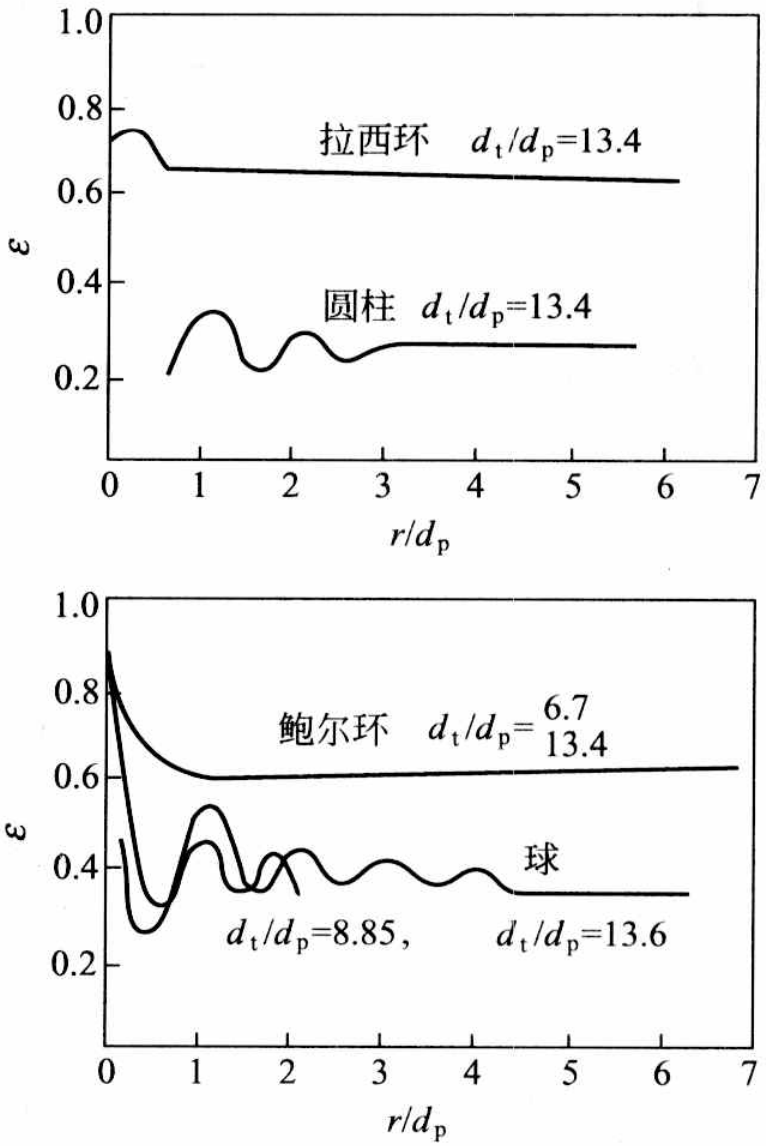
\includegraphics[width=.9\linewidth]{figures/fig7.1.png}
        \end{minipage}

\end{frame}


\begin{frame}
    \frametitle{不同形状颗粒}
    \begin{figure}[htpb]
        \centering
        \setcounter{subfigure}{0}
        \subfloat[拉西环]{
\includegraphics[height=5cm]{拉西环}}\quad
        \subfloat[鲍尔环]{
\includegraphics[height=5cm]{鲍尔环}}
    \end{figure}
\end{frame}


\begin{frame}
    \frametitle{固定床内的流体流动}

        \begin{minipage}{0.6\linewidth}
            床层空隙的径向分布是不均匀的，因而流过床层的流体，其径向流速分布也是不均匀的。
    \begin{itemize}
        \item 从床层中心处算起，随着径向位置的增大，流速增加，
        \item 在离器壁的距离等于1～2倍颗粒直径处，流速最大，然后随径向位置的增大而降低，至壁面处为零。
        \item 床层直径与颗粒直径之比越小，径向流速分布越不均匀。
    \end{itemize}
        \end{minipage}\hfill
        \begin{minipage}{0.36\linewidth}
            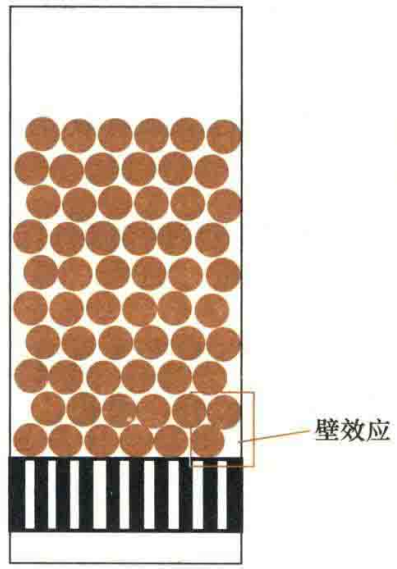
\includegraphics[width=.9\linewidth]{figures/fig7.0.png}
        \end{minipage}

\end{frame}


\begin{frame}
    \frametitle{固定床的压降}

    流体流过固定床时所产生的动量损失主要来自两方面：
    
    \begin{itemize}
        \item 流体与颗粒表面间的黏滞曳力产生的摩擦；
        \item 由不规则流体通道造成的流体湍动
    \end{itemize}
    
    当流体处于层流时，前者起主要作用；在高流速及薄床层中流动时，起主要作用的是后者。

    \begin{figure}[htpb]
        \centering
        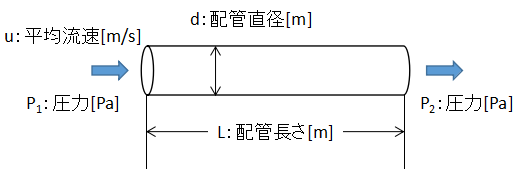
\includegraphics[width=.65\linewidth]{figures/fanning.png}
    \end{figure}

\end{frame}


\begin{frame}
    \frametitle{固定床的压降}

    流体在固定床中的流动，与空管中的流体流动相似，只是流道不规则而已。故此可将空管中流体流动的压力降计算公式修正后用于固定床。

    对于空管中的流动，可以采用Fanning范宁公式计算
    \[
        \Delta p=4 f \rho \frac{L}{d} \frac{u^{2}}{2}
    \]
    对于气固催化固定床反应器，空隙内实际流速与空塔流速之间的关系为
    \[
        u=u_{0} / \varepsilon
    \]
    修正后的固定床压力降计算公式：欧根(Ergun)公式
    \[
        \Delta p=f \frac{L_{\mathrm{r}} u_0^{2} \rho(1-\varepsilon)}{d_{\mathrm{s}} \varepsilon^{3}}
    \]
    式中颗粒直径$d_{\mathrm{s}}$按与颗粒比外表面积相等的球体的直径计算。

\end{frame}


\begin{frame}
    \frametitle{固定床的压降}

    摩擦系数$f$与雷诺数的关系如下
    \[
        f=\frac{150}{Re}+1.75
    \]
    \[
        R e=\frac{d_{\mathrm{s}} u_{0} \rho}{\mu} \times \frac{1}{1-\varepsilon}
    \]
    $\mu$为流体的黏度，\si{kg/(m.s)}；

    当$Re<10$时，流体在床层中呈层流流动，$\frac{150}{Re} \gg 1.75$，此时
    \[
        f=\frac{150}{Re}
    \]
    当$Re>1000$时，流体在床层中呈湍流流动，$\frac{150}{Re} \ll 1.75$，此时
    \[
        f=1.75
    \]

\end{frame}


\begin{frame}
    \frametitle{固定床的压降}

    由固定床压力降计算公式
    \[
        \Delta p=f \frac{L_{\mathrm{r}} u_0^{2} \rho(1-\varepsilon)}{d_{\mathrm{s}} \varepsilon^{3}}
    \]
    可知，对床层压力降影响最大的是床层的空隙率和流体的流速，两者稍有增加，都可使压力降产生较大的变化。
    
    所以，想方设法使床层的空隙增大至关重要，比如说采用粒度较大的颗粒。
    
    由公式计算得到的压力降一般是对新催化剂的预期压力降。在催化剂使用过程中会发生破损和粉化现象，使粒度减小，空隙率降低，从而使床层阻力增加。

    

\end{frame}


\begin{frame}[t]
    \frametitle{}

    \begin{example}
        在充填直径为9 mm、高为7 mm的圆柱形铁铬催化剂的固定床反应器中，0.6865 MPa下进行水煤气变换反应。反应气体的平均相对分子质量为18.96，质量速度（按空床计算）为\SI{0.936}{kg/(s.m^2)}。设床层的平均温度为689 K，反应气体的黏度等于\SI{2.5e-5}{Pa.s}。已知催化剂的颗粒密度和床层的堆密度分别为\SI{2000}{kg/m^3}及\SI{1400}{kg/m^3}。试计算单位床层高度的压力降。
    \end{example}

\end{frame}


\begin{frame}
    \frametitle{质量和热量的轴向扩散}
    对于均相系统 ， 前面曾用贝克来数来描述反应器内的轴向扩散
    \[
        P e=\frac{u L_{\mathrm{r}}}{D a}=\frac{\text { 对流传递速率 }}{\text { 扩散传递速率 }}
    \]
    这里同样采用这个准数 ， 但定性长度是以颗粒直径$d_\mathrm{p}$而不是以床层高度$L_{\mathrm{r}}$来定义 。 轴向质扩散的贝克来数为
    \[
        (P e_\mathrm{a})_\mathrm{m}=\frac{d_\mathrm{p}u}{D_\mathrm{a}}
    \]
    轴向热扩散的贝克来数则为
    \[
        (P e_\mathrm{a})_\mathrm{h}=\frac{d_\mathrm{p}u\rho C_\mathrm{p}}{\lambda_\mathrm{ea}}
    \]
    其中$\lambda_\mathrm{ea}$为床层的轴向有效导热系数 。
\end{frame}


\begin{frame}
    \frametitle{轴向质扩散的贝克来数}
    理论推导和实验测定均证明 ， 
    \begin{itemize}
      \item 当气体流过固定床且保持雷诺数$Re = d_\mathrm{p}u\rho/\mu>10$时，轴向质扩散的贝克来数$(P e_\mathrm{a})_\mathrm{m}=2$
      \item 对于液体 ，$(P e_\mathrm{a})_\mathrm{m}=0.3\sim 1$
    \end{itemize}

\end{frame}


\begin{frame}
    \frametitle{N个等体积全混釜串联模拟固定床内流体的轴向混合情况}
    定义轴向混合（或轴向扩散）距离为$l$， 则 $l=L_\mathrm{r}/N$。
    
    扩散时间$t_\mathrm{D}$与轴向扩散系数及轴向混合距离$l$间有如下关系
    \[
        t_\mathrm{D} = \frac{l^2}{2D_\mathrm{a}}
    \]
    又$t_\mathrm{D} = l/u$，所以
    \[
        t_\mathrm{D} = \frac{l^2}{2D_\mathrm{a}} = \frac{L_\mathrm{r}}{N}
    \]
    \[
        N = \frac{uL_\mathrm{r}}{2D_\mathrm{a}} = \frac{L_\mathrm{r}}{2d_\mathrm{p}}\times \frac{d_\mathrm{p}u}{D_\mathrm{a}} = \frac{L_\mathrm{r}}{2d_\mathrm{p}}(P e_\mathrm{a})_\mathrm{m}
    \]
    气体流过固定床时，$(P e_\mathrm{a})_\mathrm{m}=2$，所以
    \[
        N = \frac{L_\mathrm{r}}{d_\mathrm{p}}
    \]
\end{frame}


\begin{frame}
    \frametitle{N个等体积全混釜串联模拟固定床内流体的轴向混合情况}
    固定床内气体的流动状况用 N 个等体积的全混釜串联来描述的 ， N 是一个十分大的数 ， 等于 50 或者更大 。N 值越大越接近于活塞流 。
    \begin{itemize}
      \item 对于工业固定床反应器 ， 大多数$L_\mathrm{r}/d_\mathrm{p}$ 值远大于 50 ， 所以 ， 采用活塞流模型表示固定床内气体的流动状况是足够精确的 。
      \item 如果床层太薄将会带来较大的误差 ， 这时轴向扩散的影响不能忽略 。
    \end{itemize}
    若为非等温， 还需考虑热扩散问题 。对于非等温固定床 ， 判定能否采用活塞流模型 ， 以 ${L_\mathrm{r}}/{d_\mathrm{p}}> 150$ 作为准则比较稳妥。
    \begin{itemize}
      \item 绝大多数的工业固定床反应器都能满足这一要求。
      \item 实验室用的固定床反应器往往难于符合这个要求。
    \end{itemize}
\end{frame}


\begin{frame}
    \frametitle{径向传质与传热}
    \begin{minipage}{0.7\linewidth}
        如图为固定床反应器内进行邻二甲苯氧化反应时的床层径向温度分布图。 此图为床层进口处反应气体温度等于 357 ℃ 时的结果 ， 纵坐标为床层温度与进口温度之差 ， 横坐标则为无量纲径向位置 ， 即径向距离与床层半径之比。    
        \begin{enumerate}
        \item 图中的曲线相应于不同床层高度处的横截面径向温度分布 。
        \item 该反应为放热反应 ， 床层外壁用冷却剂冷却 ， 通过器壁以移走反应热 。
        \item 床层中心处温度最高 ， 床层外沿温度最低 。
        \item 如果是吸热反应则情况相反 ， 热量是从器壁外的载热体向床层传递 。
        \item 图中虚线与曲线的交点表示相应床层截面的平均温度 。
        \end{enumerate}
    \end{minipage}\hfill
    \begin{minipage}{0.27\linewidth}
        \begin{figure}[htpb]
            \centering
            
\includegraphics[width=\linewidth]{径向温度分布}
        \end{figure}
    \end{minipage}
\end{frame}


\begin{frame}
    \frametitle{固定床径向传热的热阻}
    \begin{figure}[htpb]
        \centering
        
\includegraphics[width=.9\linewidth]{heat}
    \end{figure}
    \begin{itemize}
      \item  球形颗粒，当$20<Re<7600$，$0.05<d_\mathrm{p}/d_\mathrm{t}<0.3$时，
      \[
        h_\mathrm{t}d_\mathrm{t}/\lambda_\mathrm{f} = 2.03Re^{0.08}\exp {(-6d_\mathrm{p}/d_\mathrm{t})}
      \]
      \item  圆柱形颗粒，当$20<Re<800$，$0.03<d_\mathrm{p}/d_\mathrm{t}<0.2$时，
      \[
        h_\mathrm{t}d_\mathrm{t}/\lambda_\mathrm{f} = 1.26Re^{0.95}\exp {(-6d_\mathrm{p}/d_\mathrm{t})}
      \]
    \end{itemize}
\end{frame}


\begin{frame}
    \frametitle{$N$个全混釜串联模拟径向混合情况}
    径向质扩散可用径向贝克来数$Pe_\mathrm{r}=d_\mathrm{p}u/D_\mathrm{r}$来描述。$D_\mathrm{r}$为径向扩散系数。当$Re>20$时，$Pe_\mathrm{r}=10$。

    对于直径为$d_\mathrm{t}$的固定床层，若用$N$个全混釜串联来模拟其径向混合情况，则
    \[
        N = \frac{d_\mathrm{t}}{L_\mathrm{r}}
    \]
    \[
        t_\mathrm{D} = \frac{l_\mathrm{r}^2}{2D_\mathrm{r}} = \frac{l_\mathrm{r}}{u}
    \]
    \[
        l_\mathrm{r} = 2D_\mathrm{r}/u
    \]
    \[
        N = \frac{ud_\mathrm{t}}{2D_\mathrm{r}} = \frac{ud_\mathrm{t}}{2d_\mathrm{p}}\times \frac{ud_\mathrm{p}}{D_\mathrm{r}} = \frac{d_\mathrm{t}}{2d_\mathrm{p}}(P e_\mathrm{r})
    \]
\end{frame}


\begin{frame}
    \frametitle{$N$个全混釜串联模拟径向混合情况}
    若$Pe_\mathrm{r}=10$，则
    \[
        N = 5\frac{d_\mathrm{t}}{d_\mathrm{p}}
    \]
    \vspace{-1em}
    \begin{enumerate}
      \item $N$不可能等于1，床层横截面上浓度也就不可能均一
      \item 径向浓度梯度总是存在的，只不过随着$d_\mathrm{t}/d_\mathrm{p}$的减小而降低
      \item 当$d_\mathrm{t}/d_\mathrm{p}$减小到5以下，床层内流体的流动将极不均匀
      \item $d_\mathrm{t}/d_\mathrm{p}$减小后容易造成流体的短路
      \item 只要$L_\mathrm{r}/d_\mathrm{p}$足够大，固定床的轴向返混是可以忽略的，但要改变$d_\mathrm{t}/d_\mathrm{p}$使径向浓度分布均匀则是困难的。
      \item 绝热式固定床反应器，完全可以不考虑径向的传热和传质。
    \end{enumerate}
\end{frame}